\documentclass{beamer}
\usepackage{amsmath}
\usepackage{hyperref}
\usepackage{listings}
\usepackage{xcolor}
\hypersetup{colorlinks=true, citecolor=blue, filecolor=blue, linkcolor=blue, urlcolor=blue}
\definecolor{codegreen}{rgb}{0,0.6,0}
\definecolor{codegray}{rgb}{0.5,0.5,0.5}
\definecolor{codepurple}{rgb}{0.58,0,0.82}
\definecolor{backcolour}{rgb}{0.95,0.95,0.92}
 
\lstdefinestyle{mystyle}{
    backgroundcolor=\color{backcolour},   
    commentstyle=\color{codegreen},
    keywordstyle=\color{magenta},
    numberstyle=\tiny\color{codegray},
    stringstyle=\color{codepurple},
    basicstyle=\ttfamily\footnotesize,
    breakatwhitespace=false,         
    breaklines=true,                 
    captionpos=b,                    
    keepspaces=true,                 
    %numbers=left,                    
    numbersep=5pt,                  
    showspaces=false,                
    showstringspaces=false,
    showtabs=false,                  
    tabsize=2
}
 
\lstset{style=mystyle}

\mode<presentation> {

% The Beamer class comes with a number of default slide themes
% which change the colors and layouts of slides. Below this is a list
% of all the themes, uncomment each in turn to see what they look like.

%\usetheme{default}
\usetheme{AnnArbor}
%\usetheme{Antibes}
%\usetheme{Bergen}
%\usetheme{Berkeley}
%\usetheme{Berlin}
%\usetheme{Boadilla}
%\usetheme{CambridgeUS}
%\usetheme{Copenhagen}
%\usetheme{Darmstadt}
%\usetheme{Dresden}
%\usetheme{Frankfurt}
%\usetheme{Goettingen}
%\usetheme{Hannover}
%\usetheme{Ilmenau}
%\usetheme{JuanLesPins}
%\usetheme{Luebeck}
%\usetheme{Madrid}
%\usetheme{Malmoe}
%\usetheme{Marburg}
%\usetheme{Montpellier}
%\usetheme{PaloAlto}
%\usetheme{Pittsburgh}
%\usetheme{Rochester}
%\usetheme{Singapore}
%\usetheme{Szeged}
%\usetheme{Warsaw}

% As well as themes, the Beamer class has a number of color themes
% for any slide theme. Uncomment each of these in turn to see how it
% changes the colors of your current slide theme.

%\usecolortheme{albatross}
%\usecolortheme{beaver}
%\usecolortheme{beetle}
%\usecolortheme{crane}
%\usecolortheme{dolphin}
%\usecolortheme{dove}
%\usecolortheme{fly}
%\usecolortheme{lily}
%\usecolortheme{orchid}
%\usecolortheme{rose}
%\usecolortheme{seagull}
%\usecolortheme{seahorse}
%\usecolortheme{whale}
%\usecolortheme{wolverine}

%\setbeamertemplate{footline} % To remove the footer line in all slides uncomment this line
\setbeamertemplate{footline}[page number] % To replace the footer line in all slides with a simple slide count uncomment this line

\setbeamertemplate{navigation symbols}{} % To remove the navigation symbols from the bottom of all slides uncomment this line
}

\usepackage{graphicx} % Allows including images
\usepackage{booktabs} % Allows the use of \toprule, \midrule and \bottomrule in tables
%\usepackage {tikz}
\usepackage{tkz-graph}
\GraphInit[vstyle = Shade]
\tikzset{
  LabelStyle/.style = { rectangle, rounded corners, draw,
                        minimum width = 2em, fill = yellow!50,
                        text = red, font = \bfseries },
  VertexStyle/.append style = { inner sep=5pt,
                                font = \normalsize\bfseries},
  EdgeStyle/.append style = {->, bend left} }
\usetikzlibrary {positioning}
%\usepackage {xcolor}
\definecolor {processblue}{cmyk}{0.96,0,0,0}
%----------------------------------------------------------------------------------------
%	TITLE PAGE
%----------------------------------------------------------------------------------------

\title[Optimization]{Numerical Optimization 02: Derivatives} % The short title appears at the bottom of every slide, the full title is only on the title page

\author{Qiang Zhu} % Your name
\institute[University of Nevada Las Vegas] % Your institution as it will appear on the bottom of every slide, may be shorthand to save space
{
University of Nevada Las Vegas\\ % Your institution for the title page
\medskip
}
\date{\today} % Date, can be changed to a custom date

\begin{document}

\begin{frame}
\titlepage % Print the title page as the first slide
\end{frame}

\begin{frame}
\frametitle{Overview} % Table of contents slide, comment this block out to remove it
\tableofcontents % Throughout your presentation, if you choose to use \section{} and \subsection{} commands, these will automatically be printed on this slide as an overview of your presentation
\end{frame}

%----------------------------------------------------------------------------------------
%	PRESENTATION SLIDES
%----------------------------------------------------------------------------------------

%------------------------------------------------

\section{Derivative}
\begin{frame}{Derivative}
The goal of optimization is to find the point that minimizes an objective function. Knowing how the value of a function changes (derivative) is useful.

 \begin{equation*}
     f(x + \Delta x) \approx f(x) + f`(x)\Delta x
 \end{equation*}
 
\begin{equation*}
    f`(x) = \frac{\Delta f(x)}{\Delta x}
\end{equation*}

Derivatives in multiple dimensions
\begin{equation*}
\textrm{\textcolor{blue}{Jacobian}}~~~~~     \nabla f(x) = \Bigg[\frac{\partial f(x)}{\partial x_1}, \frac{\partial f(x)}{\partial x_2},  \cdots \frac{\partial f(x)}{\partial x_n} \Bigg]
\end{equation*}

\begin{equation*}
\textrm{\textcolor{blue}{Hessian}}~~~~~    \nabla^2 f(x) = 
    \begin{bmatrix}
\frac{\partial^2 f(x)}{\partial x_1^2 } & \frac{\partial^2 f(x)}{\partial x_1 \partial x_2 } & \cdots \frac{\partial^2 f(x)}{\partial x_1 \partial x_n }\\
 & \vdots & \\
\frac{\partial^2 f(x)}{\partial x_n \partial x_1} & \frac{\partial^2 f(x)}{\partial x_n \partial x_2 } & \cdots \frac{\partial^2 f(x)}{\partial x_n^2 } \\
\end{bmatrix}
\end{equation*}
\end{frame}

\section{Numerical Differentiation}
\begin{frame}{Numerical Differentiation}
For practical applications, we rely on numerical methods to evaluate the derivatives.

\begin{itemize}
     \item Finite Difference Methods
     \begin{equation*}
         f`(x) \approx
    \begin{cases}
         & \frac{f(x+h)-f(x)}{h} ~~~~~~~~~~~~~~~~~\textrm{forward} \\
         & \frac{f(x+h/2)-f(x-h/2)}{h} ~~~~~~~~~~\textrm{central}\\
         & \frac{f(x)-f(x-h)}{h} ~~~~~~~~~~~~~~~~~\textrm{backward}    
     \end{cases}
     \end{equation*}
     \item Complex Step Method
     \begin{equation*}
         f`(x) = \textrm{imag}(f(x+ih)/h)
     \end{equation*}
     %\item Automatic Differentiation
\end{itemize}
\end{frame}

\begin{frame}{Finite Difference - forward}
\begin{equation*}
    f(x+h) = f(x) + \frac{f`(x)}{1!}h + \frac{f``(x)}{2!}h^2 + \frac{f```(x)}{3!}h^3 + \cdots 
\end{equation*}
\pause
We can arrange it to 

\begin{equation*}
\begin{split}
    f`(x)h &= f(x+h) - f(x) - \frac{f``(x)}{2!}h^2  - \frac{f```(x)}{3!}h^3 + \cdots \\
    f`(x) &= \frac{f(x+h) - f(x)}{h} - \frac{f``(x)}{2!}h  - \frac{f```(x)}{3!}h^2 \\
    f`(x) &= \frac{f(x+h) - f(x)}{h} + O(h)       
\end{split}
\end{equation*}
Therefore, forward difference has linear error.
\end{frame}


\begin{frame}{Finite Difference - central}
\begin{equation*}
\begin{split}
    f(x+h/2) &= f(x) + \frac{f`(x)}{1!}\frac{h}{2} + \frac{f``(x)}{2!}(\frac{h}{2})^2 + \frac{f```(x)}{3!}(\frac{h}{2})^3 + \cdots \\
    f(x-h/2) &= f(x) - \frac{f`(x)}{1!}\frac{h}{2} + \frac{f``(x)}{2!}(\frac{h}{2})^2 - \frac{f```(x)}{3!}(\frac{h}{2})^3 + \cdots \\
    f`(x) &= \frac{f(x+h/2) - f(x-h/2)}{h} + O(h^2)       
\end{split}
\end{equation*}

Therefore, central difference has quadratic error.

\end{frame}

\begin{frame}{Complex Step}
According to Taylor expansion,
\begin{equation*}
    f(x+ih) = f(x) + ihf`(x) - h^2\frac{f``(x)}{2!} - ih^3\frac{f```(x)}{3!} + \cdots 
\end{equation*}
\pause
If we take only the imaginary part,
\begin{equation*}
\begin{split}
    &\textrm{Im} (f(x+ih)) = hf`(x) -  h^3\frac{f```(x)}{3!} + \cdots \\
    &f`(x) = \frac{\textrm{Im}(f(x+ih))}{h} + h^2\frac{f```(x)}{3!} - \cdots = \frac{\textrm{Im}(f(x+ih))}{h} + O(h^2)      
\end{split}
\end{equation*}
\pause
While the real part is
\begin{equation*}
\begin{split}
		\textrm{Re}(f(x+ih)) &= f(x) - h^3\frac{f``(x)}{2!} + \cdots \\
		f(x) &= \textrm{Re}(f(x+ih)) + O(h^2)
\end{split}    
\end{equation*}
\pause
The complex step method is advantageous since 

\begin{itemize}
    \item Both $f(x)$ and $f`(x)$ can be evaluated in a single run
    \item $f`(x)$ has a quadratic error
\end{itemize}

\end{frame}

\begin{frame}{Comparison}

\begin{figure}
\centering
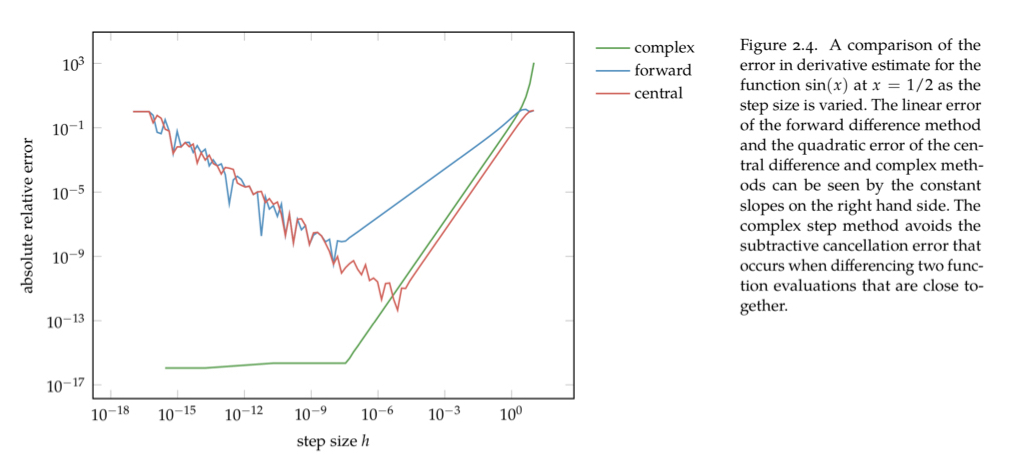
\includegraphics[width=120mm]{Figs/derivative-comparison.jpeg}
\end{figure}

\textcolor{blue}{Homework: reproduce the above figure by yourself!}
\end{frame}

\begin{frame}{Why is complex step better than central difference?}
\begin{equation*}
\begin{split}
    f(x+ih) &= u(x,h) + iv(x,h)\\
    \textrm{Im}(f(x+ih)) &= h\frac{\partial v(x, y)}{\partial y}|_{y=0} + O(h^2)
\end{split}
\end{equation*}
If $v(x,0)=0$, $f(x)=u(x,0)$. Dividing by $h$, we have f`(x)
\begin{equation*}
    \frac{\partial v(x, y)}{\partial y}|_{y=0} = \frac{\partial u(x, 0)}{\partial x}
\end{equation*}
The left side is what we used to compute the complex step. The right side is due to \textcolor{blue}{Cauchy-Riemann equation}, which is used by the finite difference. Note that two method use two different functions ($u$ and $v$).


\end{frame}

\begin{frame}{Why is complex step better than central difference?}

Consider a function $f(z) = z^2$, 
\begin{equation*}
    f(z) = z^2 = x^2 - y^2 + i2xy
\end{equation*}
The finite difference does the function $x^2$, while the complex step gives 2$x$, in the case for any $h=y>0$.
\vspace{10mm}

\pause
Try another function:
\begin{equation*}
    \cos(x+iy)=\cos(x)\textrm{cosh}(y) - i\sin(x)\textrm{sinh}(y).
\end{equation*}
The imaginary part is $−\sin(x)\sinh(y)$. For a small $y$, it gives -sin$(x)$.

\end{frame}


\section{Automatic Differentiation}
\begin{frame}{Dual numbers}
Dual numbers can be expressed mathematically by including the abstract quantity $\epsilon$, where $\epsilon^2$ is 0. So that,
\begin{equation*}
\begin{split}
    (a+b\epsilon)+(c+d\epsilon) &= (a+c) + (b+d)\epsilon\\
    (a+b\epsilon)*(c+d\epsilon) &= (ac) + (ad+bc)\epsilon
\end{split}
\end{equation*}

The function's evaluation and derivative can be expressed simultaneously in an \textcolor{blue}{exact manner}.
\begin{equation*}
\begin{split}
    f(x) &= \sum_{k=0}^\infty \frac{f^k(a)}{k!}(x-a)^k \\
    f(a+b\epsilon) &= \sum_{k=0}^\infty \frac{f^k(a)}{k!}(a+b\epsilon-a)^k
    = \sum_{k=0}^\infty \frac{f^k(a)b^k\epsilon^k}{k!}\\
    &= f(a) + bf`(a)\epsilon + \epsilon^2 \sum_{k=2}^\infty \frac{f^k(a)b^k}{k!}\epsilon^{k-2}\\
    &= f(a) + bf`(a)\epsilon
\end{split}
\end{equation*}

\end{frame}

\begin{frame}{Express a function as the computational graph}
Suppose we have a target function
\begin{equation*}
f(a, b) = \ln(ab + \textrm{max}(a, 2))
\end{equation*}

It can be expressed as
\begin{figure}
\centering
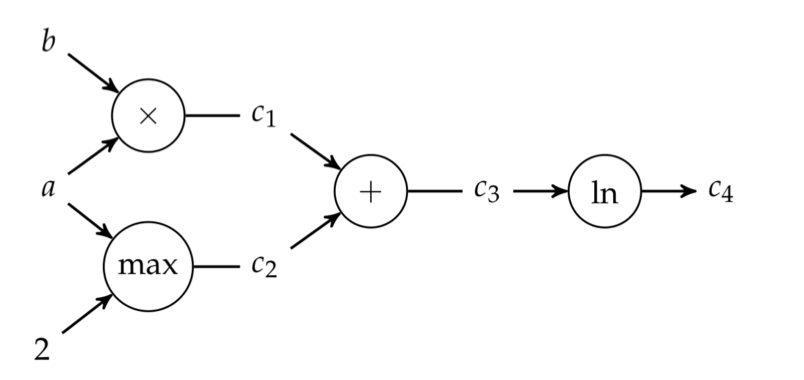
\includegraphics[width=80mm]{Figs/graph1.jpeg}
\end{figure}

\end{frame}

\begin{frame}{The derivative from the computational graph}
Suppose we have a target function
\begin{equation*}
f(a, b) = \ln(ab + \textrm{max}(a, 2))
\end{equation*}
The derivative is 
\begin{equation*}
\frac{df}{dx} = \frac{df}{dc_4}\frac{dc_4}{d_x} 
= \frac{df}{dc_4}\bigg(\frac{dc_4}{dc_3}\frac{dc_3}{dx}\bigg)
= \frac{df}{dc_4}\bigg(\frac{dc_4}{dc_3}\bigg(\frac{dc_3}{dc_2}\frac{dc_2}{dx} + \frac{dc_3}{dc_1}\frac{dc_1}{dx}\bigg)\bigg)
\end{equation*}

\begin{figure}
\centering
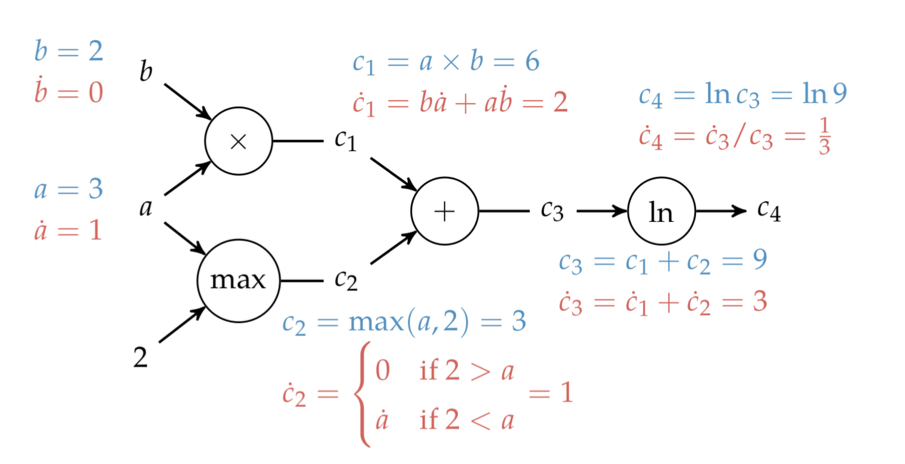
\includegraphics[width=80mm]{Figs/graph2.jpeg}
\end{figure}

\end{frame}

\section{Summary}
\begin{frame}{Summary}
    \begin{itemize}
        \item Derivatives are important for optimization. 
        \item We rely on numerical derivatives in practical optimization
        \item Finite differences are the most easy ways to compute derivative
        \item The complex step method has better accuracy
        \item Dual numbers allow the exact evaluation of function and derivative simultaneously
        \item Analytic differentiation methods include forward and reverse accumulation on computational graphs
    \end{itemize}
\end{frame}
\end{document}

